\section{Introduction}
\label{sec:introduction}

\begin{figure*}[t]
\centering
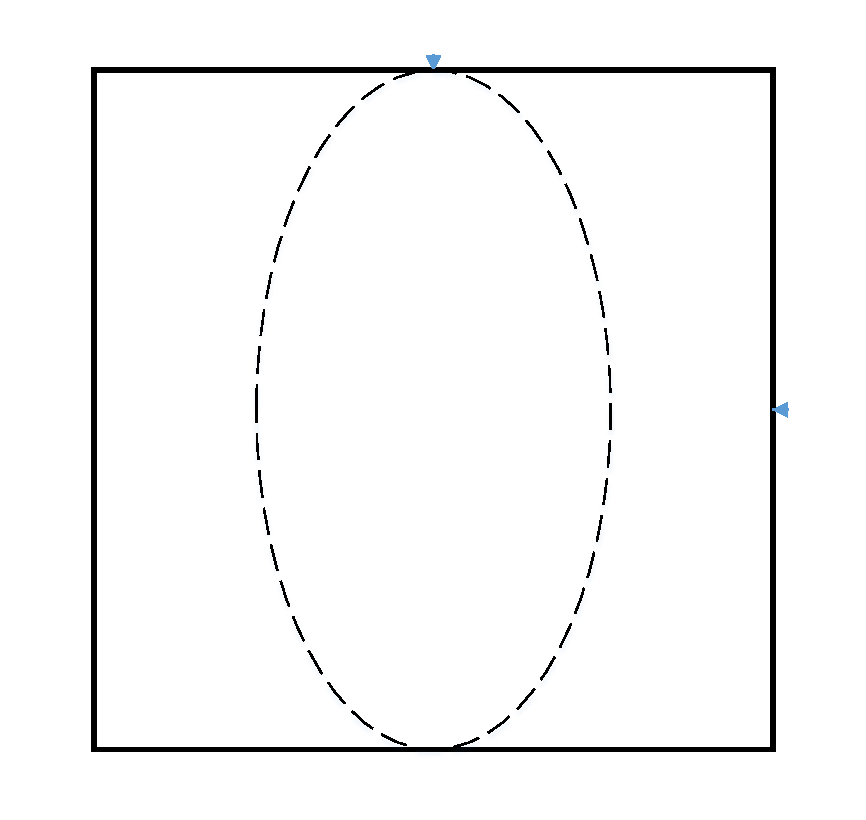
\includegraphics[width=0.3\textwidth]{temp.pdf}
\caption{ ... caption text ... }
\end{figure*}

Time series correlation is a major research topic in data mining area. 
Such correlating techniques has been applied in many real world problems.
For example, some researchers use time series correlation techniques to analysis the signal information for speech processing \cite{rabiner1993fundamentals}.
Image processing researchers also use time series correlation techniques to deal with the image retrieval problems and object detection problems \cite{yang2002detecting, sonka2014image}.
In the system diagnose area\cite{luo2014correlating,sun2014querying}, time series correlation techniques also widely used to mine the system behavior and diagnose system failures. 
Time series correlation techniques can also be used for analyzing bio-sequences (e.g DNA Sequence, etc \cite{mount2001bioinformatics} etc. 

However, in most real world problems, time series data often have different patterns (Heterogeneous time series). For example, in the area of system analysis area. 
Each performance counter can be regarded as a time series (e.g. CPU Usage, Memory Usage, etc.).
Some of the time series may be a periodical time series, but others may be a linear or random patterns. 
However, heterogeneous time series may also be correlations between each other. 
So, how to calculate the correlation between heterogeneous time series data is a challenge. 
%In addition, real world time series are all high dimensional and large scale data, how to mining such huge amount of data set is also a challenge for us.


%\textbf{System Diagnose in Online Services.}
%In real world problem of system diagnose for on-line services \cite{luo2014correlating}. On-line services, usually Large scale distributed systems, are used in a lot of industry companies, such as Google, Microsoft, and Amazon, etc. These services have the feature of (1) Large scale, (2) Distributed, (3)and available all the time $(24*7)$. As a result, when a system failure happens, it is too hard for engineers to quickly find the failure point and fix the bug. Then there will be a huge number of economic loss.
%The best way to solve the above problem is to use automatic system diagnose methods~\cite{lou2013software}. System diagnoses aims at quickly diagnosing failures by analyzing the data produced by the on-line services.
%Most of the data produced by the on-line services are Performance Counter Data (Time series data), such as CPU Usage, and Disk Usage, etc.
%As a result, evaluating the correlation between the large amount of the Performance counters (time series) is a major problem for system diagnoses.
%In sum, the task of this work is to evaluate the correlations between time series data.
%For an on-line service \cite{luo2014correlating,sun2014querying}, there are huge numbers of high dimensional time-seres produced every day.
%So, how to deal with the huge amount of high dimensional time series is a major challenge for this work.
%In addition, performance counter time series have different patterns. (Linear, Periodical, others). Like some time series is periodic, and other time series are linear time series. So, how to evaluate the correlation between the heterogeneous patterns of Time series is anther major challenge for this work.
%
%\textbf{Thread Behavior Mining in High Performance Computer.}
%High performance computers (HPC) have become enormously complex. Today, the largest systems consist of more than tens of thousands of nodes. Nodes themselves are equipped with one or more multicore microprocessors\cite{adhianto2010hpctoolkit}. 
%
%As a result, it is increasingly difficult for application developers writing complex scientific programs to attain a significant fraction of peak performance on modern microprocessor-based computer systems. 
%So, how to automatically analysis and monitoring the HPC is a major task for HPC researchers \cite{mccurdy2010memphis,tallent2009effective}.
%
%HPCToolkit\footnote{http://hpctoolkit.org/}, introduced by Dr.John Mellor-Crummey, can generate some performance information of each process (or thread if application is multithreaded.) along the time. So, each process (thread) can be represented as a time series. (Depend on which aspect of a thread to be represent, domain knowledge required) The thread change information (e.g. change from one state to another state) can directly reflect some important properties of different threads. 
%
%However, high Performance Computers often have large number (e.g. Billion Threads) of threads during running, using hash based correlation may be a good way to deal with the large scale problem of their work.
%In addition, the distribution (or Pattern) between different thread may be different, so how to deal with such heterogeneity is also a major challenge for us.

Most of the existing time series similarity measures (e.g. L1-Distance, L2-Distance \cite{han2011data}, and DTW-Distance \cite{muller2007dynamic}, etc) or correlation measures (e.g. Pearson Correlation \cite{pearson1904mathematical}, Kendall rank correlation \cite{kendall1938new}, and Spearman's rank correlation \cite{pirie1988spearman}, etc.) can not deal with such heterogeneous properties of the time series. 
Because of that, for heterogeneous time series correlating, the correlation information is often associated with the change of time series during a time period rather than a point-to-point corresponding relationship in the traditional correlation analysis techniques. 
And the existing similarity and correlation measures only consider the point to point similarity or correlation between different time series.
%In this paper, we will introduce the related research in detail in Section \ref{sec:relatedwork}.
As a result, In order to deal with heterogeneity properties of time series with different patterns. 
We proposed a change based correlation coefficient. 
The intuition of this correlation is: 

\textit{If two time series often change at the same time, they may have correlation with each other.} 

The detailed definition will be introduced in section \ref{sec:formulation}. 
Our change based correlation method firstly extract the change information of the time series data, and then use the change information to calculate the correlation coefficient between the two time series.
We also use the hashing methods speed up the correlation calculation between time series, as well as searching and clustering. 
So the computational cost of our coefficient is low, thus our method can also deal with the large scale property of the time series data.

The contribution of this paper is listed as follow:
\begin{enumerate}
\item Motivated by real applications, we investigate the correlation
problem as between heterogeneous time series (Time Series with different patterns).
To the best of our knowledge, this is the first attempt
to evaluate the correlation between time series with different patterns.

\item We proposed a correlation coefficient between heterogeneous time series, and 
use hashing method to speed up the calculating of the coefficient between time series, as well as the clustering and nearest neighbors search tasks.

\item The experiments on Synthetic data show the effectiveness and efficiency of our method.
\end{enumerate}

The rest of the paper is organized as follows: In Section 2, we introduce the problem
statement and formulation. Our approach is proposed in Section 3. The Empirical evaluation is shown in Section 4. In Section 5, we introduce some
related works. Finally, we conclude our work in Section 6.



